\documentclass[11pt]{article}

\usepackage{pdfsync}
% 1. Page Layout and Packages
\usepackage[left=0.25in,top=0.5in,right=0.25in,bottom=0.5in]{geometry} 
\usepackage{graphicx}
\usepackage[]{minted}
\usepackage{tcolorbox}


\usepackage{etoolbox}
\BeforeBeginEnvironment{minted}{\begin{tcolorbox}}%
\AfterEndEnvironment{minted}{\end{tcolorbox}}%

\usepackage{multicol} % Enables multiple columns for images in a row
\usepackage{caption}  % Allows captions outside of the figure environment

% 2. Image Path Setup
\graphicspath{{../CodeScreenshots/}{../Problem1/}{../Problem2/}{../Problem3/}}

% 3. AUTOMATION: Custom command for compact BMPs in columns
% Usage: \bmpColImage{filename}{pixelWidth}{pixelHeight}{caption}
\newcommand{\bmpColImage}[4]{
    \begin{center}
        \includegraphics[width=\linewidth, natwidth=#2, natheight=#3]{#1}
        \captionof{figure}{#4}
      %  \small(#2 $\times$ #3 pixels)
    \end{center}
}

\begin{document}

% Header Section
\noindent \textbf{Aron Rezene} \hfill \textbf{Image Processing: HW 1} \\
\noindent \today
\vspace{-5pt}
\vspace{1pt}




\begin{figure}[H]
	\centering
	
\begin{minted}{c}
#include <iostream>
#include <vector>
#include "bmp_handling.hpp"
#include "cv_bridge.hpp"
#include <opencv2/opencv.hpp>
using namespace std;

int main() {
// INITIALIZATION
string basePath = "/home/ahrgm/Projects/imgPrcsng/Content/Course_Materials/HW/HW1/";
string imgPath256 = "/home/ahrgm/Projects/imgPrcsng/imgPrcsng/src/images/lenna/lenna256.bmp";
string imgPathColor = "/home/ahrgm/Projects/imgPrcsng/imgPrcsng/src/images/lenna/lenna512_color.bmp";

BMPImage* img = readBMP(imgPath256.c_str());
BMPImage* color_img = readBMP(imgPathColor.c_str());
// Convert to OpenCV Mat for baseline comparison
cv::Mat cv_img = convertBmpToMat(img);
\end{minted}


\caption{beginning of main.cpp}
\label{figure:main_seg1}
\end{figure}


\section{Code Structure}

 The custom openCV functions used throughout the main program were declared in cv\_bridge.hpp and linked to definitions in  cv\_bridge.cpp for handling bmp files with the native OpenCV mat data type\& files. 

\begin{figure}[H]
	\centering
	
	\begin{minted}{c}
#ifndef CV_BRIDGE_HPP
#define CV_BRIDGE_HPP
#include <opencv2/opencv.hpp>
#include <string>
#include "bmp_handling.hpp"

cv::Mat convertBmpToMat(BMPImage* img);
cv::Mat resize_cv(const cv::Mat& input, int w_out, int h_out, bool use_bilinear);
cv::Mat quantize_cv(const cv::Mat& input, int bits);
double calculateMSE(const cv::Mat& img1, const cv::Mat& img2);

#endif
	\end{minted}
	
	\caption{cv\_bridge.hpp}
	\label{figure:cv_bridge}
\end{figure}

The BMPImage type definition and related functions are declared in the bmp\_handling.hpp header which is linked to function definitions in bmp\_handling.cpp .

The image file path is used as a pointer to the memory address of an image file that is read as a stream of bytes. By doing this we can pack a structure for any bmp image as specified in the BMPImage type definition. It starts with a bmp file header  occupying the first 14 bytes and an information header that occupies 40 bytes. A 1024 byte (RGBA) color pallette is then stored using the RGBQuad type definition followed by the pixel data.
A 32 bit compiler would normally store these variables each in a memory container 32 bits in size with the necessary padding. The structs are packed to ensure the memory is continuous as the file stream data is read into a struct matching the bmp header size.





\begin{figure}[H]
	\centering
	
\begin{minted}{c}
#ifndef BMP_HANDLING_H
#define BMP_HANDLING_H
#include <stdint.h>   // for handling bit sized variables

typedef struct {
uint16_t type;
uint32_t size;
uint16_t reserved1, reserved2;
uint32_t offset;
} __attribute__((packed)) BMPFileHeader;  // 14 bytes

typedef struct {
uint32_t dib_header_size;
int32_t width_px;
int32_t height_px;
uint16_t num_planes;
uint16_t bits_per_pixel;
uint32_t compression;
uint32_t image_size_bytes;
int32_t x_resolution_ppm;
int32_t y_resolution_ppm;
uint32_t num_colors;
uint32_t important_colors;
} __attribute__((packed)) BMPInfoHeader;  // 40 bytes

typedef struct {uint8_t blue, green, red, reserved;} RGBQuad;

typedef struct {
BMPFileHeader file_header;
BMPInfoHeader info_header;
RGBQuad colors[256];
unsigned char **pixels; 
} BMPImage;

BMPImage* readBMP(const char* filename);
BMPImage* createEmptyBMP(int width, int height, int bpp);
BMPImage* resize_nearest(BMPImage* input, int w_out, int h_out);
BMPImage* resize_bilinear(BMPImage* input, int w_out, int h_out);
BMPImage* extract_channel_info(BMPImage* input, int mode, int bytes); 
BMPImage* linear_quantization(BMPImage* img, int bits);

void freeBMPImage(BMPImage* img) ;
int allocatePixelMemory(BMPImage* img);
void writeBMP(const char* filename, BMPImage* img); 
void plot_histogram_gnuplot(BMPImage* img, const char* title);


#endif
\end{minted}

\caption{bmp\_handling.hpp}
\label{figure:bmpHandling}
\end{figure}










\section{Assignment}


\subsection{Problem 1: Image Resizing}
\subsubsection{Code}

\begin{figure}[H]
\begin{minted}{c}
// ==========================================
// PROBLEM 1: Resizing
// ==========================================
cout << "--- Problem 1: Resizing Comparison ---" << endl;

// --- A. Bilinear Interpolation ---
// Custom
BMPImage* bl_img = resize_bilinear(img, 64, 64);
BMPImage* restored_bl_img = resize_bilinear(bl_img, 256, 256);

writeBMP((basePath + "Problem1/imageshrunk_bilinear.bmp").c_str(), bl_img);    
writeBMP((basePath + "Problem1/imagerestored_bilinear.bmp").c_str(), restored_bl_img);

// OpenCV
cv::Mat shrunk_cv_bl = resize_cv(cv_img, 64, 64, true);
cv::Mat restored_cv_bl = resize_cv(shrunk_cv_bl, 256, 256, true);

cv::imwrite(basePath + "Problem1/cv_imageshrunk_bilinear.bmp", shrunk_cv_bl);
cv::imwrite(basePath + "Problem1/cv_imagerestored_bilinear.bmp", restored_cv_bl);

// Compare
cv::Mat restored_custom_mat_bl = convertBmpToMat(restored_bl_img);
double mse_bilinear = calculateMSE(restored_custom_mat_bl, restored_cv_bl);
cout << "MSE for Bilinear Resizing: " << mse_bilinear << endl;


// --- B. Nearest Neighbor Interpolation ---
// Custom
BMPImage* nn_img = resize_nearest(img, 64, 64);    
BMPImage* restored_nn_img = resize_nearest(nn_img, 256, 256);

writeBMP((basePath + "Problem1/imageshrunk_nn.bmp").c_str(), nn_img); 
writeBMP((basePath + "Problem1/imagerestored_nn.bmp").c_str(), restored_nn_img);

// OpenCV
cv::Mat shrunk_cv_nn = resize_cv(cv_img, 64, 64, false);
cv::Mat restored_cv_nn = resize_cv(shrunk_cv_nn, 256, 256, false);

cv::imwrite(basePath + "Problem1/cv_imageshrunk_nn.bmp", shrunk_cv_nn);
cv::imwrite(basePath + "Problem1/cv_imagerestored_nn.bmp", restored_cv_nn);

// Compare
cv::Mat restored_custom_mat_nn = convertBmpToMat(restored_nn_img);
cout << "MSE for NN: " << calculateMSE(restored_custom_mat_nn, restored_cv_nn) << endl;

\end{minted}

\caption{Problem 1 section of main.cpp}
\label{figure:Problem1}
\end{figure}



\subsubsection{Results}

% 4. MULTICOL IMPLEMENTATION: Images in a row
\begin{multicols}{2} % Change '2' to the number of images you want in a row
	
	\bmpColImage{imageshrunk_bilinear.bmp}{64}{64}{Bilinear Downsampling}
	\bmpColImage{cv_imageshrunk_bilinear.bmp}{64}{64}{OpenCV Implementation}
	
	\bmpColImage{imageshrunk_nn.bmp}{64}{64}{Nearest Neighbor Downsampling}
	\bmpColImage{cv_imageshrunk_nn.bmp}{64}{64}{OpenCV Implementation}
	
\end{multicols}

\noindent \textbf{Analysis:} There isnt much seperating either of the custom vs openCV implementations of the two algorithms. Bilinear interpolation is of course smoother but the nearest neighbor is less computationally intensive.

The resolution of all images is maintained by scaling the pixel grid to the column width. Providing the file dimensions ($256 \times 256$) ensures that XeTeX renders the BMP clearly.


% 4. MULTICOL IMPLEMENTATION: Images in a row
\begin{multicols}{2} % Change '2' to the number of images you want in a row
	
	\bmpColImage{imagerestored_bilinear.bmp}{256}{256}{Bilinear Upsampling}
	\bmpColImage{cv_imagerestored_bilinear.bmp}{256}{256}{OpenCV Implementation}
	
	\bmpColImage{imagerestored_nn.bmp}{256}{256}{Nearest Neighbor Upsampling}
	\bmpColImage{cv_imagerestored_nn.bmp}{256}{256}{OpenCV Implementation}
	
\end{multicols}

\begin{center}
	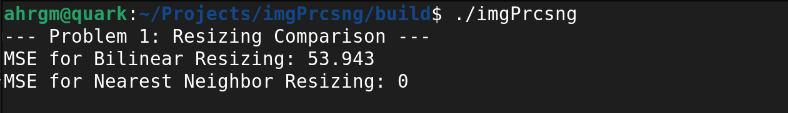
\includegraphics[width=\linewidth, natwidth=788, natheight=113]{problem1result.png}
	%\captionof{figure}{#4}
	%  \small(#2 $\times$ #3 pixels)
\end{center}

\noindent \textbf{Analysis:} The custom nearest neighbor algorithm outperforms the bilinear method for upsampled reconstruction in comparison to the openCV implementations but the bilinear method still produces the more appealing image.

\subsubsection{Function Definitions}


\begin{figure}[H]
\begin{minted}{c}
// This function uses a weighted sum for calculating pixel values
// located at new coordinate indexes. The new cordinates indexes,
// initalized as floats, are rounded to the four neighboring pixels
// indexes surrounding the interpolated point in the current pixel array.
 BMPImage* resize_bilinear(BMPImage* input, int w_out, int h_out) {

BMPImage* output = createEmptyBMP(w_out, h_out, input->info_header.bits_per_pixel);

int w_in = input->info_header.width_px;
int h_in = abs(input->info_header.height_px);

for (int i = 0; i < h_out; i++) {
for (int j = 0; j < w_out; j++) {
float x = (float)j * (float)(w_in - 1) / (float)(w_out - 1);
float y = (float)i * (float)(h_in - 1) / (float)(h_out - 1);

int x1 = (int)floor(x);
int y1 = (int)floor(y);
int x2 = (int)ceil(x);
int y2 = (int)ceil(y);

if (x2 >= w_in) x2 = w_in - 1;
if (y2 >= h_in) y2 = h_in - 1;

float wx = x - x1;
float wy = y - y1;

float q11 = (float)input->pixels[y1][x1];
float q21 = (float)input->pixels[y1][x2];
float q12 = (float)input->pixels[y2][x1];
float q22 = (float)input->pixels[y2][x2];

float r1 = q11 * (1.0f - wx) + q21 * wx;
float r2 = q12 * (1.0f - wx) + q22 * wx;
float val = r1 * (1.0f - wy) + r2 * wy;

output->pixels[i][j] = (uint8_t)round(val);
}
}
return output;
}
\end{minted}

\caption{Bilinear interpolation function in bmp\_handling.cpp}
\label{figure:Bilinear}
\end{figure}


\begin{figure}[H]
	\begin{minted}{c}
//  This function uses a scale factor of the new image dimensions to the 
//  original and assigns scaled pixel indexes (src\_x, src\_y) in the original 
//  image to regular indexes in the new image. 
BMPImage* resize_nearest(BMPImage* input, int w_out, int h_out) {

BMPImage* output = createEmptyBMP(w_out, h_out, input->info_header.bits_per_pixel);

float scale_x = (float)w_out / input->info_header.width_px;
float scale_y = (float)h_out / abs(input->info_header.height_px);

int h_in = abs(input->info_header.height_px);
int w_in = input->info_header.width_px;

for (int i = 0; i < h_out; i++) {
    for (int j = 0; j < w_out; j++) {

    int src_x = (int)floor(j / scale_x);
    int src_y = (int)floor(i / scale_y);

if (src_x >= w_in) src_x = w_in - 1;
if (src_y >= h_in) src_y = h_in - 1;

    output->pixels[i][j] = input->pixels[src_y][src_x];
}
}
return output;
}
	\end{minted}
	
	\caption{Nearest Neighbor interpolation function in bmp\_handling.cpp}
	\label{figure:Nearest}
\end{figure}






\subsection{Problem 2: Histogram Quantization }

\subsubsection{Code}

\begin{figure}[H]
\begin{minted}{c}
// ==========================================
// PROBLEM 2: Quantization
// ==========================================
cout << "\n--- Problem 2: Quantization Comparison ---" << endl;

int bits = 4; 

// Custom
BMPImage* quantized = linear_quantization(img, bits);
writeBMP((basePath + "Problem2/output_quantized.bmp").c_str(), quantized);
plot_histogram_gnuplot(quantized, "Histogram:Uniform Quantization");

// OpenCV
cv::Mat quantized_cv = quantize_cv(cv_img, bits);
cv::imwrite(basePath + "Problem2/output_quantized_cv.bmp", quantized_cv);

// Compare
cv::Mat quantized_custom_mat = convertBmpToMat(quantized);
double mse_quant = calculateMSE(quantized_custom_mat, quantized_cv);
cout << "MSE for " << bits << "-bit Quantization: " << mse_quant << endl;
\end{minted}













\caption{Problem 2 section of main.cpp}
\label{figure:Problem2}
\end{figure}



\subsubsection{Results}


\begin{multicols}{2}	 
	
	
		\bmpColImage{output_quantized.bmp}{256}{256}{OpenCV Implementation}
		\bmpColImage{output_quantized_cv.bmp}{256}{256}{OpenCV Implementation}
	%	\includegraphics[width=.75\linewidth, natwidth=256, natheight=256]{output_quantized.bmp}
	%	\captionof{figure}{Quantized image}
		%  \small(#2 $\times$ #3 pixels)


	%	\includegraphics[width=.75\linewidth, natwidth=256, natheight=256]{output_quantized_cv.bmp}
%\captionof{figure}{OpenCV Implementation}
%  \small(#2 $\times$ #3 pixels)

	
\end{multicols}

 
\begin{center}
	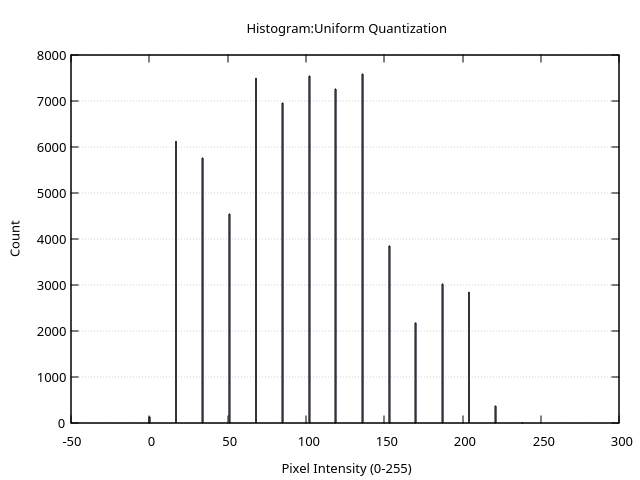
\includegraphics[width=\linewidth]{quantizedHistogram.png}
	\captionof{figure}{Histogram of quantized image}
	%  \small(#2 $\times$ #3 pixels)
\end{center}

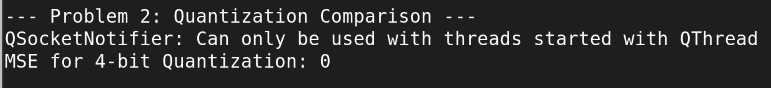
\includegraphics[width=\linewidth]{problem2result.png}
\captionof{figure}{Error from quantized image}
%  \small(#2 $\times$ #3 pixels)


\subsubsection{Function Definitions}

\begin{figure}[H]
\begin{minted}{c} 
// Maps [0-255] to 'levels' uniformly distributed values
BMPImage * linear_quantization(BMPImage* img, int bits) 
{int levels = (int)pow(2,bits);

if (levels < 2) return NULL;

float step = 255.0f / (levels - 1);

int height = abs(img->info_header.height_px);
int width = img->info_header.width_px;

BMPImage* new_img = createEmptyBMP(width, height, 8);

for (int i = 0; i < height; i++) {
for (int j = 0; j < width; j++) {
uint8_t old_pixel = img->pixels[i][j];

// 1. Determine level index
float level_idx = round(old_pixel / step);
// 2. Map back to 0-255 based on that level
uint8_t new_pixel = (uint8_t)(level_idx * step);

new_img->pixels[i][j] = new_pixel;
}
}
return new_img;
}
\end{minted}
\caption{Quantization function in bmp\_handling.cpp}
\label{figure:Quantize}
\end{figure} 


 
For the image histogram to be plotted the intensity value of each pixel in each row is counted and scans up the the column address of the 2D pixel array.


\subsection{Problem 3: Channel Extraction}

\subsubsection{Code}

\begin{figure}[H]
\begin{minted}{c}
// Extraction mode & byte indicators
int blue = 0, green = 1, red = 2, full = 3, grey = 1, clr = 3;

BMPImage* blue_mag  = extract_channel_info(color_img, blue, grey);
BMPImage* green_mag = extract_channel_info(color_img, green, grey);
BMPImage* red_mag   = extract_channel_info(color_img, red, grey);
BMPImage* grey_full = extract_channel_info(color_img, full, grey);
BMPImage* blu_mag  = extract_channel_info(color_img, blue, clr);
BMPImage* grn_mag  = extract_channel_info(color_img, green, clr);
BMPImage* rd_mag   = extract_channel_info(color_img, red, clr);
writeBMP((basePath + "Problem3/magnitude_blue.bmp").c_str(), blue_mag);    
writeBMP((basePath + "Problem3/magnitude_green.bmp").c_str(), green_mag);
writeBMP((basePath + "Problem3/magnitude_red.bmp").c_str(), red_mag);
writeBMP((basePath + "Problem3/grayscale_total.bmp").c_str(), grey_full);
writeBMP((basePath + "Problem3/color_blue.bmp").c_str(), blu_mag);
writeBMP((basePath + "Problem3/color_green.bmp").c_str(), grn_mag);
writeBMP((basePath + "Problem3/color_red.bmp").c_str(), rd_mag);

return 0;
}
\end{minted}

\caption{Problem 3 section of main.cpp}
\label{figure:Problem3}
\end{figure}


\subsubsection{Results}

\begin{multicols}{2} % Change '2' to the number of images you want in a row
	
	\bmpColImage{color.bmp}{512}{512}{Lenna in Color}
	\bmpColImage{grayscale\_total.bmp}{512}{512}{Greyscale Conversion}
	
	
	
	\bmpColImage{color\_green.bmp}{512}{512}{Green Lenna}
	\bmpColImage{color\_blue.bmp}{512}{512}{Blue Lenna}
	
	\bmpColImage{magnitude\_green.bmp}{512}{512}{Green greyscale extraction}
	\bmpColImage{magnitude\_blue.bmp}{512}{512}{Blue greyscale extraction}
		
		
	\bmpColImage{color\_red.bmp}{512}{512}{Red Lenna}
	\bmpColImage{magnitude\_red.bmp}{512}{512}{Red greyscale extraction}
	
\end{multicols}

\noindent Above are the side-by-side comparison of the processed images as a RBG image with one channel allocated versus the greyscale intensity of the same channel when the color image is converted to greyscale.

The sum of the separate greyscale intensities seems match the overall intensity see in the full grescal image after direct conversion.



\subsubsection{Function Definitions}

\begin{figure}[H]
\begin{minted}{c}
// This function separates the differnt color channels of a color input and
// uses the channel intensity to calculate the greyscale image intensity. Whe
BMPImage * extract_channel_info(BMPImage* input, int mode, int bytes) {

if (input->info_header.bits_per_pixel != 24) {
        printf("Error: Extraction requires 24-bit color input.\n");
        return NULL;
        }

int w = input->info_header.width_px;
int h = abs(input->info_header.height_px);

BMPImage * output;

if (bytes== 1){ output = createEmptyBMP(w, h, 8);

for (int i = 0; i < h; i++) {
    for (int j = 0; j < w; j++) {
// 24-bit BMP stores pixels as B, G, R
uint8_t b = input->pixels[i][j * 3 + 0];
uint8_t g = input->pixels[i][j * 3 + 1]; // Each color has an offset from the column address
uint8_t r = input->pixels[i][j * 3 + 2];

switch(mode) {
case 0: output->pixels[i][j] = (uint8_t)(0.114f*b); break; // Blue Magnitude
case 1: output->pixels[i][j] = (uint8_t)(0.587f*g); break; // Green Magnitude
case 2: output->pixels[i][j] = (uint8_t)(0.299f*r); break; // Red Magnitude
case 3: output->pixels[i][j] = (uint8_t)(0.299f*r + 0.587f*g + 0.114f*b);  // Luminosity Grayscale

break; }}}}

if (bytes == 3){ output = createEmptyBMP(w,h,24);

for (int i = 0; i < h; i++) {
    for (int j = 0; j < w; j++) {
// 24-bit BMP stores pixels as B, G, R
uint8_t b = input->pixels[i][j * 3 + 0];
uint8_t g = input->pixels[i][j * 3 + 1]; // Each color has an offset from the column address
uint8_t r = input->pixels[i][j * 3 + 2];

switch(mode) {
case 0: output->pixels[i][j*3 + 0] = b; break; // Blue Magnitude
case 1: output->pixels[i][j*3 + 1] = g; break; // Green Magnitude
case 2: output->pixels[i][j*3 + 2] = r; break; // Red Magnitude
case 3: output->pixels[i] = input->pixels[i]; // Original image 

break;}}}}

return output;
}
\end{minted}
\caption{Channel Extraction Function defined in bmp\_handling.cpp}
\label{figure:Extraction}
\end{figure}


\section{CMAKE Project File }


\begin{figure}[H]
	\begin{minted}{CMAKE}
cmake_minimum_required(VERSION 3.31)

project(imgPrcsng VERSION 1.0 LANGUAGES CXX)


find_package(OpenCV REQUIRED)

add_library(AR_bmp src/bmp_handling.cpp)

include_directories(${CMAKE_SOURCE_DIR}/include)

set(SOURCES 

main.cpp
src/bmp_handling.cpp
src/cv_bridge.cpp
)

add_executable(imgPrcsng ${SOURCES})

target_include_directories(imgPrcsng PUBLIC include src)
target_link_libraries(imgPrcsng PRIVATE AR_bmp ${OpenCV_LIBS})
\end{minted}
\end{figure}

\begin{multicols}{2}
	
	
	
	\begin{figure}[H]
		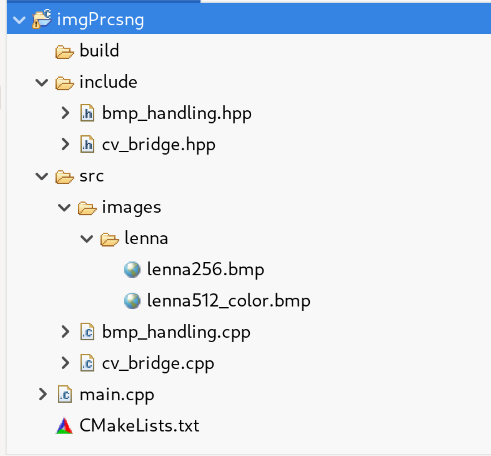
\includegraphics[width=\linewidth]{fileTree.png}
		\captionof{figure}{Project File Tree}
		%  \small(#2 $\times$ #3 pixels)
	\end{figure}
	
	
	
	
\begin{figure}[H]
\begin{minted}{bash}
cd build
cmake ..
cmake --build .
./imgPrcsng
\end{minted}
\captionof{figure}{CMake commands for building project}
\end{figure}





	
	
\end{multicols}

\end{document}